% Options for packages loaded elsewhere
\PassOptionsToPackage{unicode}{hyperref}
\PassOptionsToPackage{hyphens}{url}
\PassOptionsToPackage{dvipsnames,svgnames,x11names}{xcolor}
%
\documentclass[
  letterpaper,
  DIV=11,
  numbers=noendperiod]{scrreprt}
\usepackage{amsmath,amssymb}
\usepackage{lmodern}
\usepackage{iftex}
\ifPDFTeX
  \usepackage[T1]{fontenc}
  \usepackage[utf8]{inputenc}
  \usepackage{textcomp} % provide euro and other symbols
\else % if luatex or xetex
  \usepackage{unicode-math}
  \defaultfontfeatures{Scale=MatchLowercase}
  \defaultfontfeatures[\rmfamily]{Ligatures=TeX,Scale=1}
\fi
% Use upquote if available, for straight quotes in verbatim environments
\IfFileExists{upquote.sty}{\usepackage{upquote}}{}
\IfFileExists{microtype.sty}{% use microtype if available
  \usepackage[]{microtype}
  \UseMicrotypeSet[protrusion]{basicmath} % disable protrusion for tt fonts
}{}
\makeatletter
\@ifundefined{KOMAClassName}{% if non-KOMA class
  \IfFileExists{parskip.sty}{%
    \usepackage{parskip}
  }{% else
    \setlength{\parindent}{0pt}
    \setlength{\parskip}{6pt plus 2pt minus 1pt}}
}{% if KOMA class
  \KOMAoptions{parskip=half}}
\makeatother
\usepackage{xcolor}
\IfFileExists{xurl.sty}{\usepackage{xurl}}{} % add URL line breaks if available
\IfFileExists{bookmark.sty}{\usepackage{bookmark}}{\usepackage{hyperref}}
\hypersetup{
  colorlinks=true,
  linkcolor={blue},
  filecolor={Maroon},
  citecolor={Blue},
  urlcolor={Blue},
  pdfcreator={LaTeX via pandoc}}
\urlstyle{same} % disable monospaced font for URLs
\usepackage{color}
\usepackage{fancyvrb}
\newcommand{\VerbBar}{|}
\newcommand{\VERB}{\Verb[commandchars=\\\{\}]}
\DefineVerbatimEnvironment{Highlighting}{Verbatim}{commandchars=\\\{\}}
% Add ',fontsize=\small' for more characters per line
\usepackage{framed}
\definecolor{shadecolor}{RGB}{241,243,245}
\newenvironment{Shaded}{\begin{snugshade}}{\end{snugshade}}
\newcommand{\AlertTok}[1]{\textcolor[rgb]{0.68,0.00,0.00}{#1}}
\newcommand{\AnnotationTok}[1]{\textcolor[rgb]{0.37,0.37,0.37}{#1}}
\newcommand{\AttributeTok}[1]{\textcolor[rgb]{0.40,0.46,0.14}{#1}}
\newcommand{\BaseNTok}[1]{\textcolor[rgb]{0.68,0.00,0.00}{#1}}
\newcommand{\BuiltInTok}[1]{\textcolor[rgb]{0.00,0.46,0.62}{#1}}
\newcommand{\CharTok}[1]{\textcolor[rgb]{0.13,0.47,0.30}{#1}}
\newcommand{\CommentTok}[1]{\textcolor[rgb]{0.37,0.37,0.37}{#1}}
\newcommand{\CommentVarTok}[1]{\textcolor[rgb]{0.37,0.37,0.37}{\textit{#1}}}
\newcommand{\ConstantTok}[1]{\textcolor[rgb]{0.56,0.35,0.01}{#1}}
\newcommand{\ControlFlowTok}[1]{\textcolor[rgb]{0.00,0.46,0.62}{#1}}
\newcommand{\DataTypeTok}[1]{\textcolor[rgb]{0.68,0.00,0.00}{#1}}
\newcommand{\DecValTok}[1]{\textcolor[rgb]{0.68,0.00,0.00}{#1}}
\newcommand{\DocumentationTok}[1]{\textcolor[rgb]{0.37,0.37,0.37}{\textit{#1}}}
\newcommand{\ErrorTok}[1]{\textcolor[rgb]{0.68,0.00,0.00}{#1}}
\newcommand{\ExtensionTok}[1]{\textcolor[rgb]{0.00,0.46,0.62}{#1}}
\newcommand{\FloatTok}[1]{\textcolor[rgb]{0.68,0.00,0.00}{#1}}
\newcommand{\FunctionTok}[1]{\textcolor[rgb]{0.28,0.35,0.67}{#1}}
\newcommand{\ImportTok}[1]{\textcolor[rgb]{0.00,0.46,0.62}{#1}}
\newcommand{\InformationTok}[1]{\textcolor[rgb]{0.37,0.37,0.37}{#1}}
\newcommand{\KeywordTok}[1]{\textcolor[rgb]{0.00,0.46,0.62}{#1}}
\newcommand{\NormalTok}[1]{\textcolor[rgb]{0.00,0.46,0.62}{#1}}
\newcommand{\OperatorTok}[1]{\textcolor[rgb]{0.37,0.37,0.37}{#1}}
\newcommand{\OtherTok}[1]{\textcolor[rgb]{0.00,0.46,0.62}{#1}}
\newcommand{\PreprocessorTok}[1]{\textcolor[rgb]{0.68,0.00,0.00}{#1}}
\newcommand{\RegionMarkerTok}[1]{\textcolor[rgb]{0.00,0.46,0.62}{#1}}
\newcommand{\SpecialCharTok}[1]{\textcolor[rgb]{0.37,0.37,0.37}{#1}}
\newcommand{\SpecialStringTok}[1]{\textcolor[rgb]{0.13,0.47,0.30}{#1}}
\newcommand{\StringTok}[1]{\textcolor[rgb]{0.13,0.47,0.30}{#1}}
\newcommand{\VariableTok}[1]{\textcolor[rgb]{0.07,0.07,0.07}{#1}}
\newcommand{\VerbatimStringTok}[1]{\textcolor[rgb]{0.13,0.47,0.30}{#1}}
\newcommand{\WarningTok}[1]{\textcolor[rgb]{0.37,0.37,0.37}{\textit{#1}}}
\usepackage{longtable,booktabs,array}
\usepackage{calc} % for calculating minipage widths
% Correct order of tables after \paragraph or \subparagraph
\usepackage{etoolbox}
\makeatletter
\patchcmd\longtable{\par}{\if@noskipsec\mbox{}\fi\par}{}{}
\makeatother
% Allow footnotes in longtable head/foot
\IfFileExists{footnotehyper.sty}{\usepackage{footnotehyper}}{\usepackage{footnote}}
\makesavenoteenv{longtable}
\usepackage{graphicx}
\makeatletter
\def\maxwidth{\ifdim\Gin@nat@width>\linewidth\linewidth\else\Gin@nat@width\fi}
\def\maxheight{\ifdim\Gin@nat@height>\textheight\textheight\else\Gin@nat@height\fi}
\makeatother
% Scale images if necessary, so that they will not overflow the page
% margins by default, and it is still possible to overwrite the defaults
% using explicit options in \includegraphics[width, height, ...]{}
\setkeys{Gin}{width=\maxwidth,height=\maxheight,keepaspectratio}
% Set default figure placement to htbp
\makeatletter
\def\fps@figure{htbp}
\makeatother
\setlength{\emergencystretch}{3em} % prevent overfull lines
\providecommand{\tightlist}{%
  \setlength{\itemsep}{0pt}\setlength{\parskip}{0pt}}
\setcounter{secnumdepth}{-\maxdimen} % remove section numbering
\KOMAoption{captions}{tableheading}
\makeatletter
\makeatother
\makeatletter
\@ifpackageloaded{caption}{}{\usepackage{caption}}
\AtBeginDocument{%
\renewcommand*\contentsname{Table of contents}
\renewcommand*\listfigurename{List of Figures}
\renewcommand*\listtablename{List of Tables}
\renewcommand*\figurename{Figure}
\renewcommand*\tablename{Table}
}
\@ifpackageloaded{float}{}{\usepackage{float}}
\floatstyle{ruled}
\@ifundefined{c@chapter}{\newfloat{codelisting}{h}{lop}}{\newfloat{codelisting}{h}{lop}[chapter]}
\floatname{codelisting}{Listing}
\newcommand*\listoflistings{\listof{codelisting}{List of Listings}}
\makeatother
\makeatletter
\@ifpackageloaded{caption}{}{\usepackage{caption}}
\@ifpackageloaded{subcaption}{}{\usepackage{subcaption}}
\makeatother
\makeatletter
\makeatother
\ifLuaTeX
  \usepackage{selnolig}  % disable illegal ligatures
\fi

\author{}
\date{}

\begin{document}

\hypertarget{monthly-no2-timeseries}{%
\chapter*{Monthly NO2 Timeseries}\label{monthly-no2-timeseries}}
\addcontentsline{toc}{chapter}{Monthly NO2 Timeseries}

\hypertarget{timeseries-of-monthly-no2-using-rioxarray-satsarch-and-stackstac}{%
\section{\texorpdfstring{2016-2022 Timeseries of Monthly NO2 Using
\texttt{rioxarray}, \texttt{satsarch} and
\texttt{stackstac}}{2016-2022 Timeseries of Monthly NO2 Using rioxarray, satsarch and stackstac}}\label{timeseries-of-monthly-no2-using-rioxarray-satsarch-and-stackstac}}

\begin{Shaded}
\begin{Highlighting}[]
\ImportTok{import}\NormalTok{ rioxarray}
\ImportTok{import}\NormalTok{ stackstac}
\ImportTok{from}\NormalTok{ satsearch }\ImportTok{import}\NormalTok{ Search}
\end{Highlighting}
\end{Shaded}

\begin{Shaded}
\begin{Highlighting}[]
\NormalTok{stac\_api\_url }\OperatorTok{=} \StringTok{\textquotesingle{}https://staging{-}stac.delta{-}backend.xyz/\textquotesingle{}}
\NormalTok{china\_bbox }\OperatorTok{=}\NormalTok{ [}
    \FloatTok{73.675}\NormalTok{,}
    \FloatTok{18.198}\NormalTok{,}
    \FloatTok{135.026}\NormalTok{,}
    \FloatTok{53.459}
\NormalTok{]}
\NormalTok{datetime }\OperatorTok{=} \StringTok{"2000{-}01{-}01T00:00:00Z/2022{-}01{-}02T00:00:00Z"}
\NormalTok{collection }\OperatorTok{=} \StringTok{\textquotesingle{}no2{-}monthly\textquotesingle{}}

\NormalTok{search }\OperatorTok{=}\NormalTok{ Search.search(}
\NormalTok{    url}\OperatorTok{=}\NormalTok{stac\_api\_url,}
\NormalTok{    bbox}\OperatorTok{=}\NormalTok{china\_bbox,}
\NormalTok{    datetime}\OperatorTok{=}\NormalTok{datetime,}
\NormalTok{    collections}\OperatorTok{=}\NormalTok{[collection],}
\NormalTok{    limit}\OperatorTok{=}\DecValTok{1000}
\NormalTok{)}
\NormalTok{items }\OperatorTok{=}\NormalTok{ search.items()}
\end{Highlighting}
\end{Shaded}

\begin{verbatim}
url is https://staging-stac.delta-backend.xyz/search
headers is None
kwargs is {'limit': 1000, 'bbox': [73.675, 18.198, 135.026, 53.459], 'datetime': '2000-01-01T00:00:00Z/2022-01-02T00:00:00Z', 'collections': ['no2-monthly']}
\end{verbatim}

\begin{Shaded}
\begin{Highlighting}[]
\BuiltInTok{len}\NormalTok{(items)}
\end{Highlighting}
\end{Shaded}

\begin{verbatim}
73
\end{verbatim}

\begin{Shaded}
\begin{Highlighting}[]
\NormalTok{stack }\OperatorTok{=}\NormalTok{ stackstac.stack(items)}
\end{Highlighting}
\end{Shaded}

\begin{Shaded}
\begin{Highlighting}[]
\NormalTok{stack}
\end{Highlighting}
\end{Shaded}

\begin{verbatim}
<xarray.DataArray 'stackstac-a8afebb458dddd242ccfecc9f369d38d' (time: 73,
                                                                band: 1,
                                                                y: 1800, x: 3600)>
dask.array<fetch_raster_window, shape=(73, 1, 1800, 3600), dtype=float64, chunksize=(1, 1, 1024, 1024), chunktype=numpy.ndarray>
Coordinates:
  * time            (time) datetime64[ns] 2016-01-01 2016-02-01 ... 2022-01-01
    id              (time) <U46 'OMI_trno2_0.10x0.10_201601_Col3_V4-no2-month...
  * band            (band) <U11 'cog_default'
  * x               (x) float64 -180.0 -179.9 -179.8 ... 179.7 179.8 179.9
  * y               (y) float64 90.0 89.9 89.8 89.7 ... -89.6 -89.7 -89.8 -89.9
    proj:epsg       int64 4326
    proj:bbox       object {180.0, -180.0, 90.0, -90.0}
    proj:shape      object {1800, 3600}
    proj:geometry   object {'type': 'Polygon', 'coordinates': [[[-180.0, 90.0...
    proj:transform  object {0.1, 0.0, -0.1, 1.0, -180.0, 90.0}
    epsg            int64 4326
Attributes:
    spec:        RasterSpec(epsg=4326, bounds=(-180.0, -90.0, 180.0, 90.0), r...
    crs:         epsg:4326
    transform:   | 0.10, 0.00,-180.00|\n| 0.00,-0.10, 90.00|\n| 0.00, 0.00, 1...
    resolution:  0.1
\end{verbatim}

\begin{Shaded}
\begin{Highlighting}[]
\CommentTok{\# Subset to Bounding Box for China}
\NormalTok{subset }\OperatorTok{=}\NormalTok{ stack.rio.clip\_box(}
\NormalTok{    minx}\OperatorTok{=}\NormalTok{china\_bbox[}\DecValTok{0}\NormalTok{],}
\NormalTok{    miny}\OperatorTok{=}\NormalTok{china\_bbox[}\DecValTok{1}\NormalTok{],}
\NormalTok{    maxx}\OperatorTok{=}\NormalTok{china\_bbox[}\DecValTok{2}\NormalTok{],}
\NormalTok{    maxy}\OperatorTok{=}\NormalTok{china\_bbox[}\DecValTok{3}\NormalTok{]}
\NormalTok{)}
\NormalTok{subset}
\end{Highlighting}
\end{Shaded}

\begin{verbatim}
<xarray.DataArray 'stackstac-a8afebb458dddd242ccfecc9f369d38d' (time: 73,
                                                                band: 1,
                                                                y: 354, x: 614)>
dask.array<getitem, shape=(73, 1, 354, 614), dtype=float64, chunksize=(1, 1, 354, 535), chunktype=numpy.ndarray>
Coordinates:
  * time            (time) datetime64[ns] 2016-01-01 2016-02-01 ... 2022-01-01
    id              (time) <U46 'OMI_trno2_0.10x0.10_201601_Col3_V4-no2-month...
  * band            (band) <U11 'cog_default'
  * x               (x) float64 73.7 73.8 73.9 74.0 ... 134.7 134.8 134.9 135.0
  * y               (y) float64 53.5 53.4 53.3 53.2 53.1 ... 18.5 18.4 18.3 18.2
    proj:epsg       int64 4326
    proj:bbox       object {90.0, 180.0, -90.0, -180.0}
    proj:shape      object {1800, 3600}
    proj:geometry   object {'type': 'Polygon', 'coordinates': [[[-180.0, 90.0...
    proj:transform  object {0.1, 0.0, 1.0, -0.1, -180.0, 90.0}
    epsg            int64 4326
    spatial_ref     int64 0
Attributes:
    spec:        RasterSpec(epsg=4326, bounds=(-180.0, -90.0, 180.0, 90.0), r...
    resolution:  0.1
\end{verbatim}

\begin{Shaded}
\begin{Highlighting}[]
\CommentTok{\# select the band default}
\NormalTok{data\_band }\OperatorTok{=}\NormalTok{ subset.sel(band}\OperatorTok{=}\StringTok{\textquotesingle{}cog\_default\textquotesingle{}}\NormalTok{)}
\NormalTok{data\_band}
\end{Highlighting}
\end{Shaded}

\begin{verbatim}
<xarray.DataArray 'stackstac-a8afebb458dddd242ccfecc9f369d38d' (time: 73,
                                                                y: 354, x: 614)>
dask.array<getitem, shape=(73, 354, 614), dtype=float64, chunksize=(1, 354, 535), chunktype=numpy.ndarray>
Coordinates:
  * time            (time) datetime64[ns] 2016-01-01 2016-02-01 ... 2022-01-01
    id              (time) <U46 'OMI_trno2_0.10x0.10_201601_Col3_V4-no2-month...
    band            <U11 'cog_default'
  * x               (x) float64 73.7 73.8 73.9 74.0 ... 134.7 134.8 134.9 135.0
  * y               (y) float64 53.5 53.4 53.3 53.2 53.1 ... 18.5 18.4 18.3 18.2
    proj:epsg       int64 4326
    proj:bbox       object {90.0, 180.0, -90.0, -180.0}
    proj:shape      object {1800, 3600}
    proj:geometry   object {'type': 'Polygon', 'coordinates': [[[-180.0, 90.0...
    proj:transform  object {0.1, 0.0, 1.0, -0.1, -180.0, 90.0}
    epsg            int64 4326
    spatial_ref     int64 0
Attributes:
    spec:        RasterSpec(epsg=4326, bounds=(-180.0, -90.0, 180.0, 90.0), r...
    resolution:  0.1
\end{verbatim}

\begin{Shaded}
\begin{Highlighting}[]
\CommentTok{\# Group data into months}
\NormalTok{no2\_months }\OperatorTok{=}\NormalTok{ data\_band.groupby(}\StringTok{\textquotesingle{}time\textquotesingle{}}\NormalTok{)}
\end{Highlighting}
\end{Shaded}

\begin{Shaded}
\begin{Highlighting}[]
\CommentTok{\# Average over entire spatial bounding box for each month}
\NormalTok{monthly\_mean\_no2 }\OperatorTok{=}\NormalTok{ no2\_months.mean(dim}\OperatorTok{=}\NormalTok{(}\StringTok{\textquotesingle{}x\textquotesingle{}}\NormalTok{, }\StringTok{\textquotesingle{}y\textquotesingle{}}\NormalTok{))}
\end{Highlighting}
\end{Shaded}

\begin{Shaded}
\begin{Highlighting}[]
\OperatorTok{\%\%}\NormalTok{time}
\NormalTok{monthly\_mean\_no2.plot()}
\end{Highlighting}
\end{Shaded}

\begin{verbatim}
CPU times: user 6.72 s, sys: 2.58 s, total: 9.29 s
Wall time: 35.8 s
\end{verbatim}

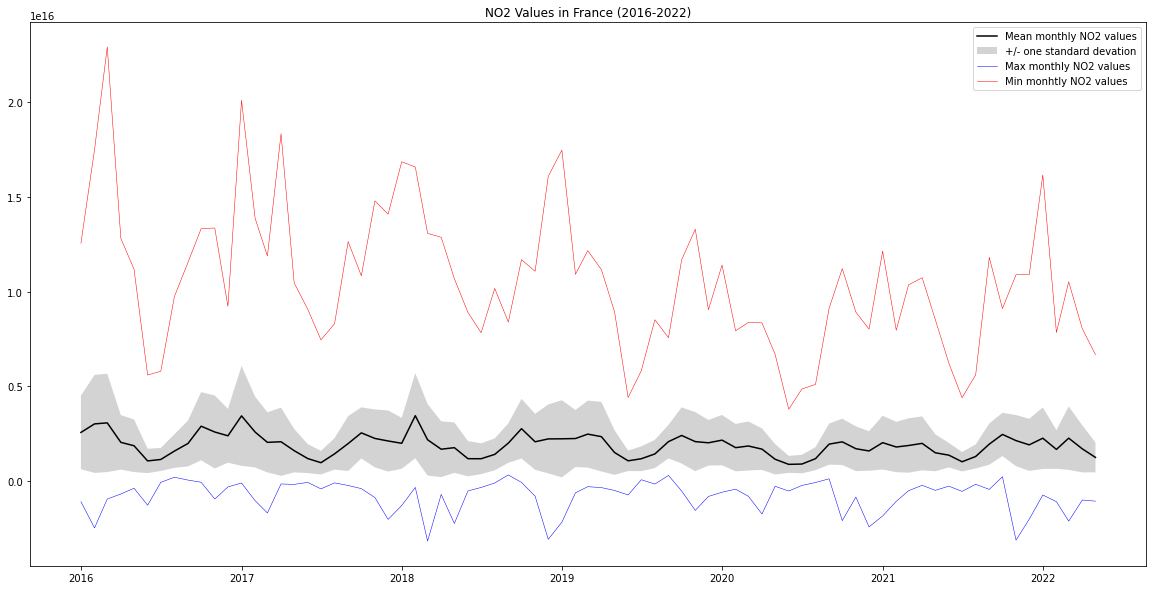
\includegraphics{no2-timeseries_files/figure-pdf/cell-11-output-2.png}

\end{document}
